\documentclass{beamer}

\pdfmapfile{+sansmathaccent.map}


\mode<presentation>
{
	\usetheme{Warsaw} % or try Darmstadt, Madrid, Warsaw, Rochester, CambridgeUS, ...
	\usecolortheme{seahorse} % or try seahorse, beaver, crane, wolverine, ...
	\usefonttheme{serif}  % or try serif, structurebold, ...
	\setbeamertemplate{navigation symbols}{}
	\setbeamertemplate{caption}[numbered]
} 


%%%%%%%%%%%%%%%%%%%%%%%%%%%%
% itemize settings

\definecolor{mypaleblue}{RGB}{240, 240, 255}
\definecolor{mylightblue}{RGB}{120, 150, 255}
\definecolor{myblue}{RGB}{90, 90, 255}
\definecolor{mygblue}{RGB}{70, 110, 240}
\definecolor{mydarkblue}{RGB}{0, 0, 180}
\definecolor{myblackblue}{RGB}{40, 40, 120}

\definecolor{mygreen}{RGB}{0, 200, 0}
\definecolor{mydarkgreen}{RGB}{0, 120, 0}
\definecolor{mygreen2}{RGB}{245, 255, 230}

\definecolor{mygray}{gray}{0.8}
\definecolor{mygray2}{RGB}{130, 130, 130}
\definecolor{mydarkgray}{RGB}{80, 80, 160}
\definecolor{mylightgray}{RGB}{160, 160, 160}

\definecolor{mydarkred}{RGB}{160, 30, 30}
\definecolor{mylightred}{RGB}{255, 150, 150}
\definecolor{myred}{RGB}{200, 110, 110}
\definecolor{myblackred}{RGB}{120, 40, 40}

\definecolor{mypink}{RGB}{255, 30, 80}
\definecolor{myhotpink}{RGB}{255, 80, 200}
\definecolor{mywarmpink}{RGB}{255, 60, 160}
\definecolor{mylightpink}{RGB}{255, 80, 200}
\definecolor{mydarkpink}{RGB}{155, 25, 60}

\definecolor{mydarkcolor}{RGB}{60, 25, 155}
\definecolor{mylightcolor}{RGB}{130, 180, 250}

\setbeamertemplate{itemize items}[default]

\setbeamertemplate{itemize item}{\color{myblackblue}$\blacksquare$}
\setbeamertemplate{itemize subitem}{\color{mydarkblue}$\blacktriangleright$}
\setbeamertemplate{itemize subsubitem}{\color{mygray}$\blacksquare$}

\setbeamercolor{palette quaternary}{fg=white,bg=mygblue} %mydarkgray
\setbeamercolor{titlelike}{parent=palette quaternary}

\setbeamercolor{palette quaternary2}{fg=white,bg=mygblue}%black myblue
\setbeamercolor{frametitle}{parent=palette quaternary2}

\setbeamerfont{frametitle}{size=\Large,series=\scshape}
\setbeamerfont{framesubtitle}{size=\normalsize,series=\upshape}


%%%%%%%%%%%%%%%%%%%%%%%%%%%%
% block settings

%\setbeamercolor{block title}{bg=red!50,fg=black}
%\setbeamercolor{block title}{bg=mylightblue,fg=black}
\setbeamercolor{block title}{bg=myblackblue,fg=white}

\setbeamercolor*{block title example}{bg=mygreen!40!white,fg=black}

\setbeamercolor*{block body example}{fg= black,
	bg= mygreen2}


%%%%%%%%%%%%%%%%%%%%%%%%%%%%
% URL settings
\hypersetup{
	colorlinks=false,
	linkcolor=blue,
	filecolor=blue,      
	urlcolor=blue,
}

%%%%%%%%%%%%%%%%%%%%%%%%%%

\renewcommand{\familydefault}{\rmdefault}

\usepackage{amsmath}
\usepackage{mathtools}

\usepackage{subcaption}

\usepackage{qrcode}

\newcommand{\bo}[1] {\mathbf{#1}}
\newcommand{\R}{\mathbb{R}} 
\newcommand{\T}{^\top}     



\newcommand{\mydate}{Spring 2025}

\newcommand{\mygit}{\textcolor{blue}{\href{https://github.com/SergeiSa/Computational-Intelligence-2025}{github.com/SergeiSa/Computational-Intelligence-2025}}}

\newcommand{\myqr}{ \textcolor{black}{\qrcode[height=1.5in]{https://github.com/SergeiSa/Computational-Intelligence-2025}}
}

\newcommand{\myqrframe}{
	\begin{frame}
		\centerline{Lecture slides are available via Github, links are on Moodle:}
		\bigskip
		\centerline{\mygit}
		\bigskip
		\myqr
	\end{frame}
}


\newcommand{\bref}[2] {\textcolor{blue}{\href{#1}{#2}}}



%%%%%%%%%%%%%%%%%%%%%%%%%%%%
% code settings

\usepackage{listings}
\usepackage{color}
% \definecolor{mygreen}{rgb}{0,0.6,0}
% \definecolor{mygray}{rgb}{0.5,0.5,0.5}
\definecolor{mymauve}{rgb}{0.58,0,0.82}
\lstset{ 
	backgroundcolor=\color{white},   % choose the background color; you must add \usepackage{color} or \usepackage{xcolor}; should come as last argument
	basicstyle=\footnotesize,        % the size of the fonts that are used for the code
	breakatwhitespace=false,         % sets if automatic breaks should only happen at whitespace
	breaklines=true,                 % sets automatic line breaking
	captionpos=b,                    % sets the caption-position to bottom
	commentstyle=\color{mygreen},    % comment style
	deletekeywords={...},            % if you want to delete keywords from the given language
	escapeinside={\%*}{*)},          % if you want to add LaTeX within your code
	extendedchars=true,              % lets you use non-ASCII characters; for 8-bits encodings only, does not work with UTF-8
	firstnumber=0000,                % start line enumeration with line 0000
	frame=single,	                   % adds a frame around the code
	keepspaces=true,                 % keeps spaces in text, useful for keeping indentation of code (possibly needs columns=flexible)
	keywordstyle=\color{blue},       % keyword style
	language=Octave,                 % the language of the code
	morekeywords={*,...},            % if you want to add more keywords to the set
	numbers=left,                    % where to put the line-numbers; possible values are (none, left, right)
	numbersep=5pt,                   % how far the line-numbers are from the code
	numberstyle=\tiny\color{mygray}, % the style that is used for the line-numbers
	rulecolor=\color{black},         % if not set, the frame-color may be changed on line-breaks within not-black text (e.g. comments (green here))
	showspaces=false,                % show spaces everywhere adding particular underscores; it overrides 'showstringspaces'
	showstringspaces=false,          % underline spaces within strings only
	showtabs=false,                  % show tabs within strings adding particular underscores
	stepnumber=2,                    % the step between two line-numbers. If it's 1, each line will be numbered
	stringstyle=\color{mymauve},     % string literal style
	tabsize=2,	                   % sets default tabsize to 2 spaces
	title=\lstname                   % show the filename of files included with \lstinputlisting; also try caption instead of title
}

%%%%%%%%%%%%%%%%%%%%%%%%%%%%
% tikz settings

\usepackage{tikz}
\tikzset{every picture/.style={line width=0.75pt}}

%%%%%%%%%%%%%%%%%%%%%%%%%%%%



\newcommand{\Zo}[2] {\left\langle {#1},{#2}
	\right\rangle}

\title{Model-predictive control}
\subtitle{Computational Intelligence, Extra 1}
\author{by Sergei Savin}
\centering
\date{\mydate}



\begin{document}
\maketitle


\begin{frame}{Content}

\begin{itemize}
\item  Dynamical systems, linearization, discretization
\item Trajectory planning
\item OCP / MPC for DT-LTV
\item Zonotopes and explicit MPC
	\begin{itemize}
		\item  Definition
		\item  Operations
		\item Containment, convex hull
		\item MPC
	\end{itemize}
\end{itemize}

\end{frame}





\begin{frame}{Dynamical system}
	%\framesubtitle{How do we know the state?}
	\begin{flushleft}
		
		Given a dynamical system described as an ODE:
		
		\begin{equation}
			\label{eq:ODE}
			\dot{\bo{x}} = \bo{f}(\bo{x}, \bo{u}),
		\end{equation} 
		
		we can find a pair of time functions - control law $\bo{u}^* = \bo{u}^*(t)$ and state trajectory $\bo{x}^* = \bo{x}^*(t)$, that conform with the ODE \eqref{eq:ODE}. The problem of finding such pair is called \emph{trajectory planning}.
		
		\bigskip
		
		\begin{example}
			
			A forced spring-damper dynamics is described with the following state-space model:
			
			$$
			\begin{bmatrix}
				\dot x_1 \\ \dot x_2
			\end{bmatrix}
			= 
			\begin{bmatrix}
				0 & 1 \\ -k & -\mu
			\end{bmatrix}
			\begin{bmatrix}
				x_1 \\ x_2
			\end{bmatrix}
		+
		\begin{bmatrix}
			0 \\ u
		\end{bmatrix}
			$$
		\end{example}
		
	\end{flushleft}
\end{frame}



\begin{frame}{Linearization}
	%\framesubtitle{How do we know the state?}
	\begin{flushleft}
		
		Once we found control law $\bo{u}^* = \bo{u}^*(t)$ and state trajectory $\bo{x}^* = \bo{x}^*(t)$ we can find \emph{linearization} of the dynamical system, via Taylor expansion:
		%
		\begin{equation}
			\bo{f}(\bo{x}, \bo{u}) \approx 
			\bo{f}(\bo{x}^*, \bo{u}^*)
			+
			\frac{\partial \bo{f}}{\partial \bo{x}} (\bo{x} - \bo{x}^*)
			+
			\frac{\partial \bo{f}}{\partial \bo{u}} (\bo{u} - \bo{u}^*)
		\end{equation} 
		
		We denote Jacobian matrices as $\bo{A}$ and $\bo{B}$, giving as \emph{state matrix} and \emph{control matrix}
		%
		\begin{align}
			\bo{A}(t) = \frac{\partial \bo{f}(\bo{x}, \bo{u})}{\partial \bo{x}}, \\
			\bo{B}(t) = \frac{\partial \bo{f}(\bo{x}, \bo{u})}{\partial \bo{u}},
		\end{align}
		
		...for a time-varying linear system (LTV):
		%
		\begin{equation}
			\dot{\bo{e}} = \bo{A}(t) \bo{e} + \bo{B}(t) \bo{u}
		\end{equation} 
		
	\end{flushleft}
\end{frame}



\begin{frame}{Discretization}
	%\framesubtitle{How do we know the state?}
	\begin{flushleft}
		
		Linear system $\dot{\bo{e}} = \bo{A}(t) \bo{e} + \bo{B}(t) \bo{u}$ is represented as \emph{a continuous-time} model. We could re-write it as a discrete time model:
		
		\begin{equation}
			\bo{z}_{i+1} = \bar{\bo{A}}_i \bo{z}_i + \bar{\bo{B}}_i \bo{u}_i
		\end{equation} 
		
		This can be done via a number of methods (with different assumptions), such as \emph{zero-order hold} or by exact discretization.
		
	\end{flushleft}
\end{frame}




\begin{frame}{Trajectory planning as optimization}
	% \framesubtitle{Parameter estimation}
	\begin{flushleft}
		
		We can formulate the trajectory planning as an \emph{optimal control problem} (OCP):
		
		\begin{equation}
			\begin{aligned}
				& \underset{\bo{x}(t), \bo{u}(t)}{\text{minimize}}
				& & l_f(\bo{x}(t_f)) + \int\limits_{t_0}^{t_f} l \left( \bo{x}(t), \bo{u}(t) \right) dt, \\
				& \text{subject to:}
				& & \dot{\bo{x}} = 
				\bo{f}(\bo{x}, \bo{u}) \\
				& & & \bo{x}(t_0) = 
				\bo{x}_0 \\
				& & & \bo{x}(t) \in \text{workspace} \\
				& & & \bo{u}_{min} \leq \bo{u}(t) \leq \bo{u}_{max}
			\end{aligned}
		\end{equation}
		
		This is an optimization problem with continuous variables and there are no solvers that can solve it (in a general case). We can replace the continuous time variables with a finite number of parameters. This is called \emph{transcription}.
		
	\end{flushleft}
\end{frame}




\begin{frame}{OCP for discrete LTV: MPC as QP}
	% \framesubtitle{Parameter estimation}
	\begin{flushleft}
		
		Given a discrete linear system $\bo{x}_{i+1} = \bo{A}_i \bo{x}_i + \bo{B}_i \bo{u}_i$ and a quadratic objective, we can formulate the OCP as a quadratic program:
		%
		\begin{equation}
			\label{eq:QP}
			\begin{aligned}
				& \underset{\bo{x}_i, \bo{u}_i}{\text{minimize}}
				& & \bo{x}_N\T \bo{Q}_N \bo{x}_N + \sum\limits_{i=1}^{N-1} \left( \bo{x}_i\T \bo{Q}_i \bo{x}_i + \bo{u}_i\T \bo{R}_i \bo{u}_i \right), \\
				& \text{subject to:}
				& & \bo{x}_{i+1} = \bo{A}_i \bo{x}_i + \bo{B}_i \bo{u}_i \\
				& & & \bo{F}_i \bo{x}_i \leq \bo{h}_i \\
				& & & \bo{u}_{min}  \leq \bo{u}_i \leq \bo{u}_{max}
			\end{aligned}
		\end{equation}
		
		This can be solved efficiently; setting $N$ to be relatively small we make it into a \emph{receding horizon} \emph{model-predictive control} (MPC). 
		
		Solution to \eqref{eq:QP} gives us a sequence of control actions $\bo{u}_i$.
		
	\end{flushleft}
\end{frame}



\begin{frame}{MPC as QP}
	% \framesubtitle{Parameter estimation}
	\begin{flushleft}
		
		\begin{itemize}
			\item If problem \eqref{eq:QP} has no inequality constraints, it can be solved analytically.
			
			\item Robust control (uncertain input or uncertain model) with MPC based on quadratic program is easy to implement.
			
			\item Linear-quadratic regulator (LQR) problems are closely related. LQR allows us to obtain linear control law $\bo{u} = \bo{K}\bo{x}$. LQR does not depend on knowing exact initial conditions and can be solved as a single SDP (semidefinite program).
			
			\item Given a trajectory of a non-linear system, we can linearize its dynamics along the trajectory, and then find control law either via MPC or LQR.
		\end{itemize}
		
	\end{flushleft}
\end{frame}



\begin{frame}
	
	\centering{\huge Zonotopes and explicit MPC}
	
\end{frame}


\begin{frame}{Zonotopes}
	% \framesubtitle{Parameter estimation}
	\begin{flushleft}
		
		A zonotope can be defined as a point-symmetric set in $n$-dimensional space, described as a center $c \in \mathbb{R}^n $ and $p$ generators $g^{(i)} \in \mathbb{R}^n, \ i \in \{1,...,p\}$; the latter can be presented as columns of matrix $G \in \mathbb{R}^{n \times p}$:
		%
		\begin{equation} 
			\label{eq_zonotope_def}
			\mathbb{Z} = \Zo{c}{G} = \{c + \sum_{i=1}^p \beta_i g^{(i)} :  -1 \leq \beta_i \leq 1 \}
		\end{equation}
		%
		where $\beta_i$ are scalar multipliers. Eq. \eqref{eq_zonotope_def} defines a \emph{vector zonotope}. 
		
	\end{flushleft}
\end{frame}



\begin{frame}{Zonotopes}
	% \framesubtitle{Parameter estimation}
	\begin{flushleft}
		
		\begin{figure}
			\centering
			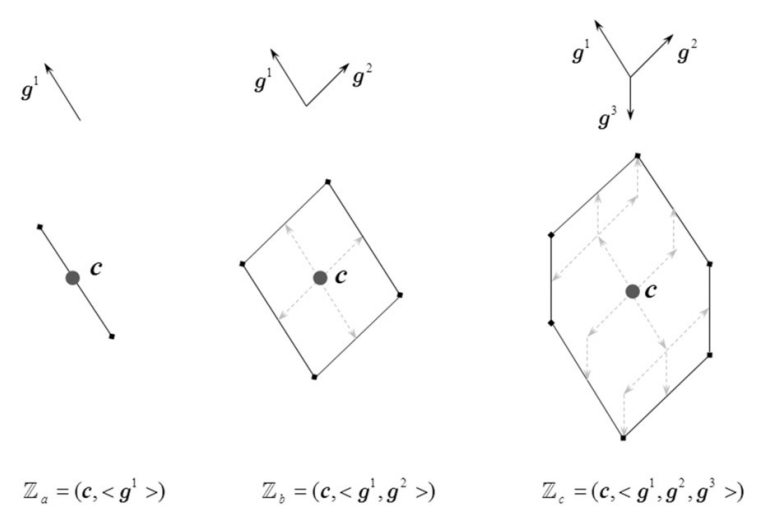
\includegraphics[width=0.7\linewidth]{zonotopes}
			\caption{An example of a zonotope;  \bref{https://journals.sagepub.com/doi/abs/10.1177/0954410018810255?journalCode=piga}{source}.}
			\label{fig:zonotopes}
		\end{figure}
		
		
	\end{flushleft}
\end{frame}




\begin{frame}{Algebraic Operations on Vector Zonotopes}
	% \framesubtitle{Parameter estimation}
	\begin{flushleft}
		
		Vector zonotopes are closed under addition and linear transformation:
		%
		\begin{equation} 
			\label{eq_zonotope_addition}
			\Zo{x}{X}+\Zo{y}{Y} = \Zo{x+y}{X+Y}
		\end{equation}
		\begin{equation} 
			\label{eq_zonotope_linear_tranform}
			A\Zo{c}{G} = \Zo{Ac}{AG},
		\end{equation}
		%
		where $A$ is a linear operator.
	\end{flushleft}
\end{frame}



\begin{frame}{Algebraic Operations on Vector Zonotopes}
	% \framesubtitle{Parameter estimation}
	\begin{flushleft}
		
		Minkowski sum for vector zonotopes is defined as:
		%
		\begin{equation}
			\label{eq:MinkowskiDef}
			\Zo{x}{X} \oplus \Zo{y}{Y} = \Zo{x + y}{(X, Y)}
		\end{equation}
		%
		where notation $(X, Y)$ refers to horizontal matrix concatenation. 
		
		\bigskip
		
		We can define the addition of a vector zonotope and a vector as follows:
		%
		\begin{equation} 
			\label{eq_zonotope_vector_addition}
			\Zo{c}{G}+v = \Zo{c+v}{G}
		\end{equation}
		
		
	\end{flushleft}
\end{frame}



\begin{frame}{Zonotope Containtment}
	% \framesubtitle{Parameter estimation}
	\begin{flushleft}
		
		
		Given two zonotopes $\mathbb{X}$ = $\langle x,X \rangle$ and $\mathbb{Y}$ = $\langle y,Y \rangle$, where $X \in \mathbb{R}^{n \times n_x}$, $Y \in \mathbb{R}^{n \times n_y}$, if there exists $\Gamma \in \mathbb{R}^{n_y \times n_x}$ and $\beta \in \mathbb{R}^{n_y}$, such that:
		%
		\begin{equation}
			\label{eq:containment}
			X = Y\Gamma, \ y - x = Y\beta, \  ||(\Gamma,\beta)||_\infty \leq 1
		\end{equation}
		%
		then zonotope $\mathbb{X}$ is contained in zonotope $\mathbb{Y}$. This method is convenient, as it requires solving a single linear program.
		
	\end{flushleft}
\end{frame}


\begin{frame}{Approximating convex hull of two zonotopes}
	% \framesubtitle{Parameter estimation}
	\begin{flushleft}
		
		The following is an approximation of the convex hull of two zonotopes $\mathbb{X} = \langle x,X \rangle$ and $\mathbb{Y} = \langle y,Y \rangle$:
		%
		\begin{equation}
			\label{eq_convhull}
			\text{Co}(\mathbb{X}, \mathbb{Y}) \subseteq 
			\Zo{\frac{x + y}{2}}
			{\left(
				\frac{X + Y}{2},\frac{x - y}{2},\frac{X - Y}{2}
				\right)}
		\end{equation}
		
		This method is conservative and computationally inexpensive. Most importantly for our purpose, it can be incorporated in a convex optimization problem formulation as an equality constraint. 
		
		
	\end{flushleft}
\end{frame}




\begin{frame}{State propagation}
	% \framesubtitle{Parameter estimation}
	\begin{flushleft}
		
		We can describe how the state changes with respect to time:
		%
		\begin{equation}
			x_{k+1}  = A_k x_k + B_k u_k + d_k + w_k
		\end{equation}
		%
		where $w_k \in \mathbb{W}_k$ is random external disturbance.
		
	\end{flushleft}
\end{frame}





\begin{frame}{MPC: Uncertain input and certain model (1)}
	% \framesubtitle{Parameter estimation}
	\begin{flushleft}
		
		State propagation problem can be described as an evolution (propagation) of the initial zonotope $\mathbb{X}_1$:
		%
		\begin{equation}
			\label{eq:LTV_zonotopes}
				\mathbb{X}_{k+1}  = (A_k \mathbb{X}_k + B_k \mathbb{U}_k + d_k) \oplus \mathbb{W}_k
		\end{equation}
		%
		where 
		$\mathbb{X}_k = \Zo{\bar{x}_k}{G_k}$, 
		$\mathbb{U}_k = \Zo{\bar{u}_k}{\theta_k}$, 
		and 
		$\mathbb{W}_k = \Zo{0_{n \times 1}}{W(k)}$ are zonotopes representing state, control actions, and process noise, 
		$G_k      \in \mathbb{R}^{n \times p}$, 
		$\theta_k \in \mathbb{R}^{m \times p}$, and 
		$W(k)      \in \mathbb{R}^{n \times n_w}$ are generators or these zonotopes, 
		$\bar{x}_k      \in \mathbb{R}^{n}$ and 
		$\bar{u}_k \in \mathbb{R}^{m}$ 
		are their centers.  
		
		
	\end{flushleft}
\end{frame}


\begin{frame}{MPC: Uncertain input and certain model (2)}
	% \framesubtitle{Parameter estimation}
	\begin{flushleft}
		
		We can re-write the zonotope propagation as:
		%
		\begin{equation}
			\begin{cases}
				G_{k+1}  = (A_k G_k + B_k \theta_k, \ \ W_k)
				\\
				\bar{x}_{k+1}  = A_k \bar{x}_k + B_k \bar{u}_k + d_k
			\end{cases}
		\end{equation}
		
		Disturbance $w_k \in \mathbb{W}_k$ act on the system on each time step; therefore the order of the zonotopes $\mathbb{X}_k$ grows on each time step, unless order reduction techniques are employed. 
		
		\bigskip
		
		We know that state is given as $x = \bar{x}_k + G_k \beta$ and control is $u = \bar{u}_k + \theta_k \beta$. Expressing $\beta$ from the first and substituting it to the second, we find control law as $u_k = K_k (x_k - \bar{x}_k) + \bar{u}_k$, where $K_k = \theta_k G_k^+$.
		
	\end{flushleft}
\end{frame}



\myqrframe


\end{document}
